\chapter{Generative Adversarial Networks - Partie théorique}

Après avoir appris à manipuler correctement les réseaux perceptrons simples, nous nous sommes intéressés à la structure de \textbf{Generative Adversarial Networks}, qui a constitué le cœur du projet, et son enjeu majeur. 

La naissance du GAN se place dans un contexte de recherche de moyens innovants et efficaces de génération de données arbitraires. Dans l'ère de l'information, les données constituent une ressource fondamentale, et la capacité d'en générer facilement de nouvelles représente un pan entier de la recherche, si ce n'est plusieurs. Le GAN sont une solution à base de réseaux à apprentissage semi-supervisés, dont l'objectif est de générer des données arbitraires en extrapolant à partir de données initialement fournies.

Dans ce chapitre, nous décrirons qualitativement le fonctionnement attendu des GANs et leur théorie, puis nous détaillerons les aspects plus techniques et mathématiques du problème. 

\section{Description du fonctionnement des \textit{Generative Adversarial Networks}}

Le GAN est une structure qui fait intervenir deux réseaux placés en compétition, qui vont s'émuler mutuellement afin d'atteindre un optimum, ceci en partant de rien. Les GAN représentent un domaine de recherche qui s'est ouvert en 2014 avec la publication d'un article de Ian Goodfellow \cite{goodfellow_generative_2014}.

En 2014,l'équipe de Ian Goodfellow publie dans NIPS un article intitulé \textbf{Generative Adversarial Nets}, dans lequel il décrit une nouvelle structure censée répondre au problème de génération de donnée. Cette structure est fondée sur l'entraînement simultané de deux réseaux neuronaux en compétition, respectivement nommés \textbf{Générateur} et \textbf{Discriminateur}.  

% A compléter avec l'article en question

\subsection{GAN - Idée générale}

Pour commencer, on souhaite obtenir un réseau qui soit capable de générer sur commande des données 
\begin{itemize}
    \item Pertinentes par rapport aux contraintes qu'on lui impose (exemple : on souhaite pouvoir obtenir un réseau qui dessine spécifiquement des moutons, et non un réseau qui dessine n'importe quoi comme bon lui semble)
    \item Variées, c'est à dire que les données générées sont différentes deux a deux
    \item Réalistes, voire indiscernables de données réelles aux yeux d'un humain \\
\end{itemize} 

En résumé on souhaite construire un réseau (nommé dans toute la suite \textbf{Générateur}) qui modélise une projection d'un ensemble d'entrée vers l'ensemble des données réalistes et pertinentes vis-à-vis des contraintes imposées, et dont l'image ne soit pas réduite à un point de cet ensemble.

Résumée de cette façon, la tâche semble extraordinairement ardue, c'est pourquoi la structure fait appel à un second réseau (nommé \textbf{Discriminateur} dans toute la suite). En effet, la difficulté principale liée aux réseaux de neurones est l'apprentissage. Dans ce cas en particulier, la difficulté majeure  est de caractériser ce qu'est une donnée de synthèse \"pertinente et réaliste, voire indiscernable d'une donnée réelle\"; car s'il est très facile de distinguer à l’œil une image de mouton de n'importe quoi d'autre, il est extrêmement difficile de construire un critère mathématique permettant de distinguer les images de mouton des autres. Or c'est ce critère dont nous avons besoin pour faire apprendre correctement à notre \textbf{Générateur}.

Cependant, nous avons vus avec les perceptrons et la base de données MNIST qu'il était parfaitement possible d'obtenir un réseau de neurones modélisant avec une grande précision des critères visuels, que l'on serait bien incapables d'exprimer mathématiquement. Il est par exemple impossible d'écrire analytiquement ce qu'est un chiffre manuscrit, mais il est possible de générer un réseau de neurones qui sache discriminer les chiffres manuscrits des autres images. Ainsi, en déléguant à un second réseau la responsabilité de modéliser le critère selon lequel nous voulons que nos données soient générées (exemple: on ne veut générer que des images de mouton, on va faire apprendre au \textbf{Discriminateur} à différencier un mouton de toutes les autres images possibles), on résout le (premier) problème majeur qui se pose. 

\subsection{Des réseaux en compétition}

Le GAN va donc faire intervenir deux réseaux, dont l'un sert seulement à rendre possible l'apprentissage de l'autre. Le \textbf{Discriminateur} a pour unique rôle de modéliser le critère que l'on souhaite utiliser; son apprentissage se fait donc de la même manière que tout ce qui a été fait jusqu'ici, en apprentissage supervisé. C'est un réseau dont l'entrée est de la dimension des données que l'on souhaite construire, et dont la sortie est un réel entre 0 et 1, caractérisant la certitude du réseau que l'entrée qui lui été donnée est une donnée réelle ou non. Plus précisément, pour une entrée donnée, plus la sortie est proche de 1, plus le \textbf{Discriminateur} est convaincu que l'entrée est une donnée réelle, et non de synthèse. Son objectif est donc de sortir 1 pour toute entrée réelle, et 0 pour toute donnée de synthèse.

Le \textbf{Générateur} de son côté est le réseau qui doit générer des données synthétiques suffisamment convaincantes pour que le \textbf{Discriminateur} ne puisse les différencier des données réelles. Sa sortie est donc naturellement de la dimension des données qu'on souhaite construire. L'entrée du \textbf{Générateur} est un bruit (blanc) à partir duquel le réseau doit construire une donnée convaincante. Le \textbf{Générateur} est donc un réseau qui réalise une projection de l'ensemble d'entrée vers l'ensemble des données \"suffisamment convaincantes pour tromper un humain\". Passer un bruit en entrée permet d'obtenir des sorties variées. On comprend cependant que, le réseau réalisant un calcul déterministe, la dimension de la sorties est nécessairement inférieure à la dimension de l'entrée. Pour être certain d'obtenir un ensemble de sortie aussi grand que possible, on s'assurera toujours d'avoir un ensemble d'entrée de dimension suffisamment grande. \\

\begin{example} Cas des images de mouton

On souhaite obtenir un réseau qui génère des images $28 \times 28$ de moutons, suffisamment réalistes pour ne pouvoir être distinguées de réelles photos de moutons. On souhaite également observer de la variation dans ces images (avoir plein de moutons différents). 

L'ensemble de sortie du \textbf{Générateur} est donc un ensemble inclus dans l'ensemble des images $28 \times 28$ et qui contient toutes les images que le \textbf{Générateur} considère comme étant des moutons réalistes. Pour être certain que l'ensemble d'entrée soit de dimension au moins aussi importante que l'ensemble de sortie, on mettra en entrée du réseau un bruit blanc de dimension $28 \times 28$. On est certain de cette façon que la taille de l'ensemble d'entrée n'impose pas de restriction sur les sorties. 

\end{example}

\begin{example} Génération du chiffre 8
On peut schématiser 
\begin{figure}[h]
\begin{center}
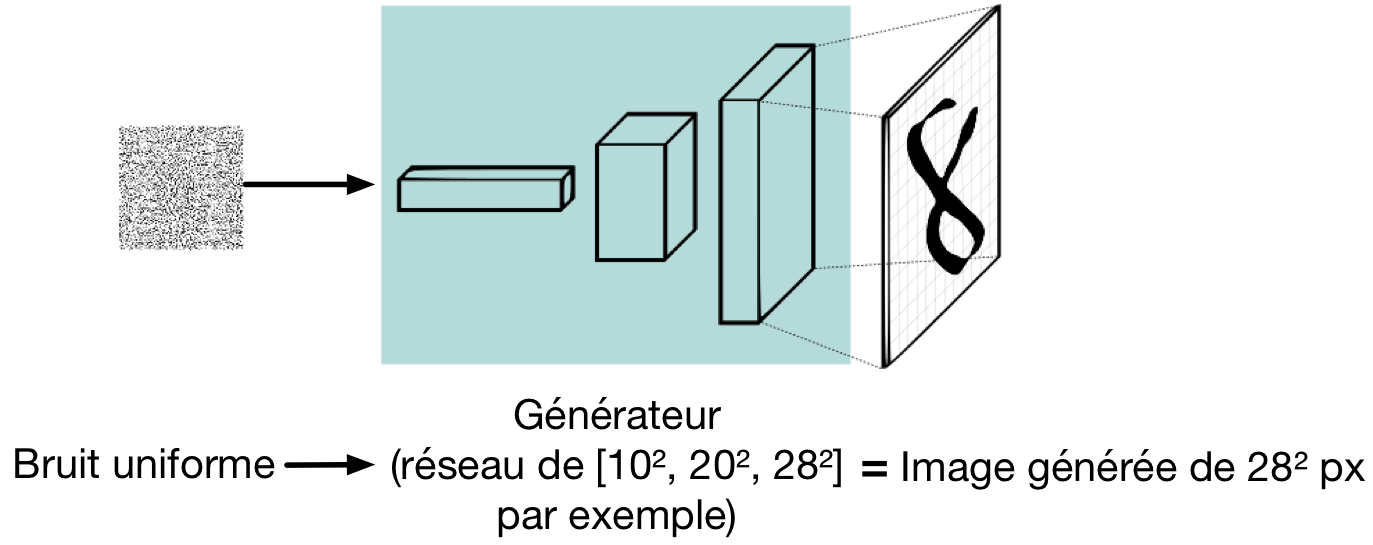
\includegraphics[width=0.5\textwidth]{images/Colloque/generateur.png}\caption{Génération du chiffre 8 par un générateur $100\times 400\times 784$}
\end{center}
\end{figure} 
\end{example}
\section{Discriminateur et Générateur}
\subsection{Notations}
On note \theta^{(D)} et \theta^{(G)} les paramètres des réseaux, représentant les valeurs de la matrice de poids et de biais de chacun des réseaux.
On dispose de deux fonctions de coûts, notées $J^{(D)}(\theta^{(D)}, \theta^{(G)})$ et $J^{(G)}(\theta^{(D)}, \theta^{(G)})$, représentant respectivement les fonctions de coûts du Discriminateur et du Générateur. Dans leur notation, on montre bien que chacune d'elle dépendent des paramètres de chacun des deux réseaux. En effet, le Discriminateur apprend à discerner les fausses images issues du générateur des vrais images, tandis que le générateur apprend grâce aux indications fournies par le Discriminateur. 
On note $z$ l'entrée du générateur (du bruit blanc multidimensionnel), $x$ une image réelle (issue d'une banque d'image), $G(z)$ la sortie du générateur (une image générée) et enfin $D(x)$ et $D(G(z))$ la sortie du discriminateur comportant en entrée respectivement une image réel et une image générée (le score donné respectivement à une image réelle et à une image générée. 
$x$ est alors une variable d'observation tandis que $z$ est une variable \textit{indirecte}. 
D et G représentent alors des fonctions (différentiables) de paramètres \theta^{(D)} et \theta^{(G)}.
\begin{remarque}
On notera que le bruit n'est pas nécessairement présent uniquement sur la première couche, il peut être présent quel que soit la couche. Il a été implémenté avec succès (voir \textit{NoisyLayer} dans \cite{barrios_gan_2018}), et utilisé avec succès par le groupe Salamandre \cite{bouvier_dyvoire_dessine-moi_2018}
\end{remarque}
\subsection{Théorie des jeux et équilibre de Nash}
\subsubsection{$D(G(z)) = D(x) = \frac{1}{2}$ : un premier critère d'optimalité}
Comme toute fonction de coût, le discriminateur cherchera au cours de l'apprentissage à réduire la fonction de coût $J^{(D)}(\theta^{(D)}, \theta^{(G)})$, en n'ayant de contrôle que sur \theta^{(D)}. De même, le générateur cherchera à réduire la fonction de coût $J^{(G)}(\theta^{(D)}, \theta^{(G)})$, en n'ayant de contrôle que sur \theta^{(G)}. 
La solution à ce problème peut se traduire en théorie des jeux. On obtient alors un équilibre de Nash. 

\subsection{Les différentes distributions statistiques impliquées}
Les distributions que l'on considère sont $p{data}, p_{model} et p_{G}, ....

\section{Les fonctions de coût, l'apprentissage}

\subsection{Les différentes fonctions de coût}
\paragraph{Discriminateur}
Le discriminateur n'a, dans le cas du GAN classique, qu'une fonction de coût qui soit utilisée : 
$J^{(D)}(\theta^{(D)}, \theta^{(G)}) = -\frac{1}{2}\E_{x~p_{data}}\log{D(x)}-\frac{1}{2}\E_{z}\log{1-D(G(z))}$

$-\frac{1}{2}\E_{x~p_{data}}\log{D(x)}$ correspond à la capacité de D à reconnaître les vraies images, tandis que -\frac{1}{2}\E_{z}\log{1-D(G(z))}$ correspond à la capacité de D à reconnaître les résultats de G.

\paragraph{Générateur}
Le générateur peut prendre plusieurs fonctions de coût. On a implémenté le MinMax, l'heuristique non saturante et le maximum de vraisemblance (aussi appelée KL-Divergence). 

\subsection{Apprentissage par récompense ou par punition ?}
\begin{figure}[h]
\begin{center}
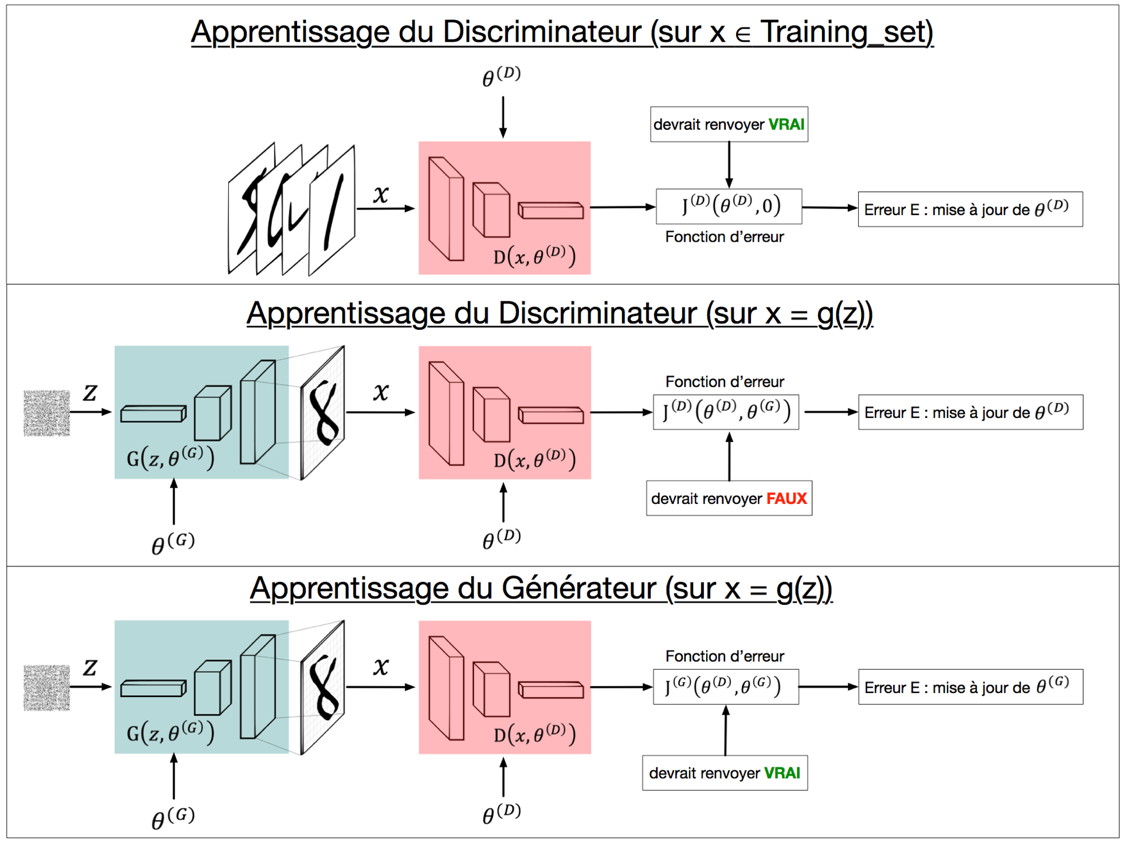
\includegraphics[width=0.5\textwidth]{images/Colloque/apprentissage.png}\caption{Les 3 types d'apprentissages successifs appliqués au GAN}
\end{center}
\end{figure} 
\end{example}
\subsection{Quand un réseau prend le pas sur l'autre}
